
Explain the specific challenges in the strip detector that are parameterized and modeled
in our case.

\subsubsection{DCDC converter}

The DCDC converter (FEAST) supplies a low-voltage (1.5~V) current to the ABC130 and HCC front-end
chips on the module.
The efficiency of the FEAST depends on its temperature as well as the output (load) current
load delivered to the front-end chips. To correctly model the FEAST efficiency, experimental
measurements are performed to characterize the dependence, and fitted with a functional form with
sufficient parameters to ensure reasonable agreement. Figure~\ref{fig:feast_eff} depicts the
FEAST efficiency data and the parameterization used in the model.

\begin{figure}[ht]
\centering
\subfloat[] {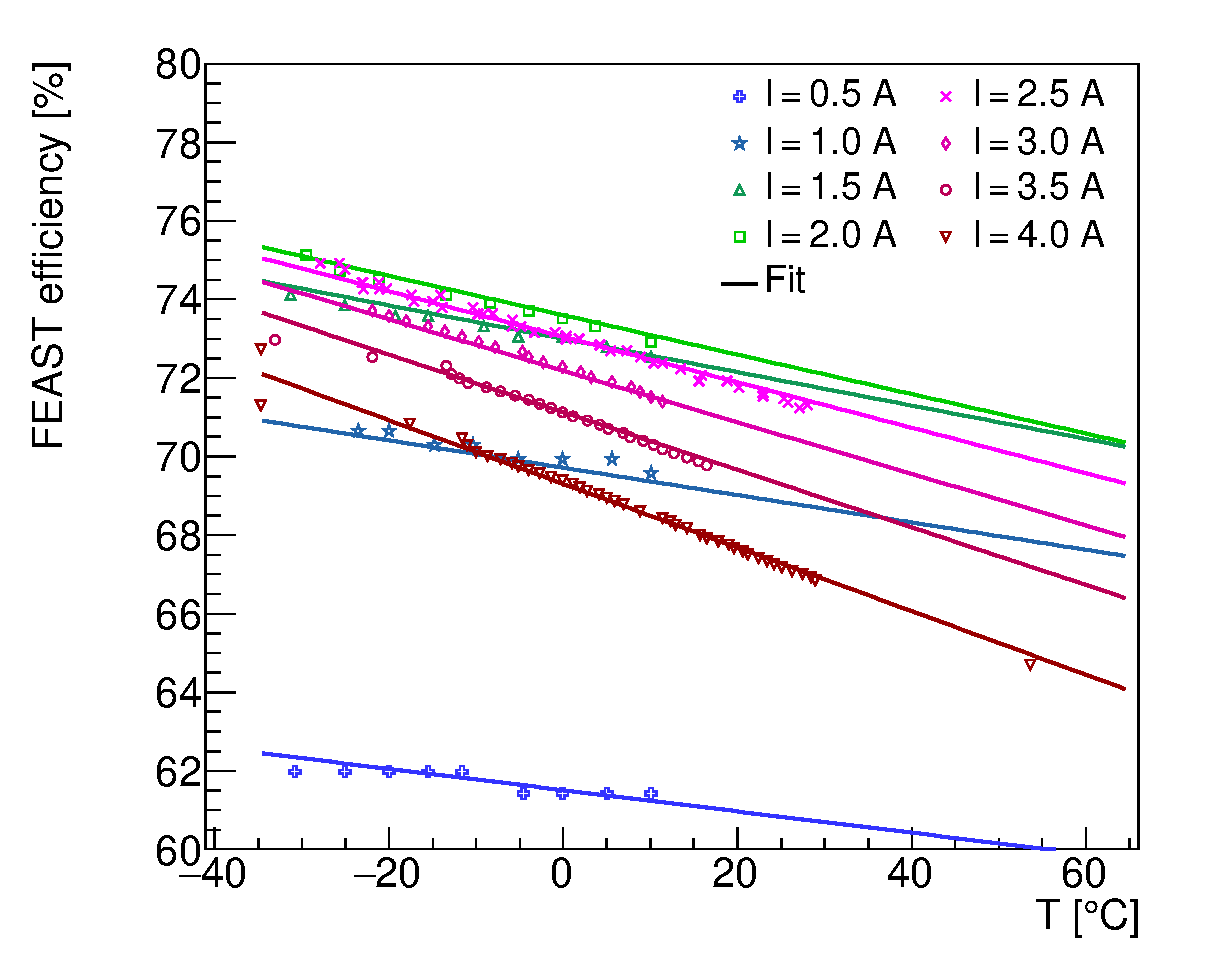
\includegraphics[width=0.49\linewidth]{figures/FeastEfficiency_isoCurrent.eps}}
\subfloat[] {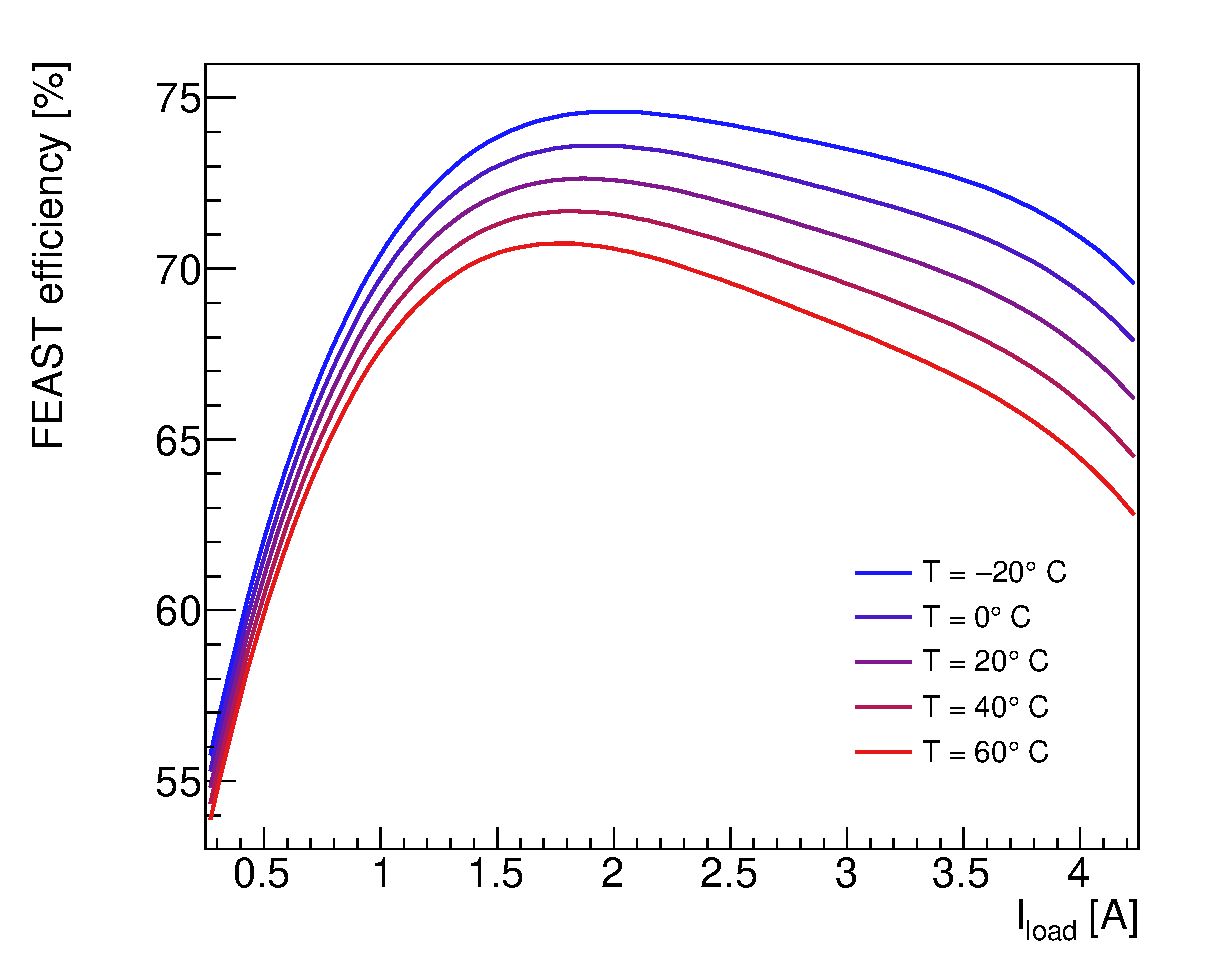
\includegraphics[width=0.49\linewidth]{figures/FeastEfficiency.eps}}
\caption{The FEAST efficiency model based on experimental data. (a) The experimental data points
characterizing the FEAST efficiency are plotted as dots and color coded for load current. The data is
compared to the analytic fit, evaluated in curves of equal current. (b) The same analytic fit,
presented as a function of current load for curves of equal temperature.
}
\label{fig:feast_eff}
\end{figure}


\subsubsection{Digital current increase of chips using 130~nm CMOS technology}

\begin{figure}[ht]
\centering
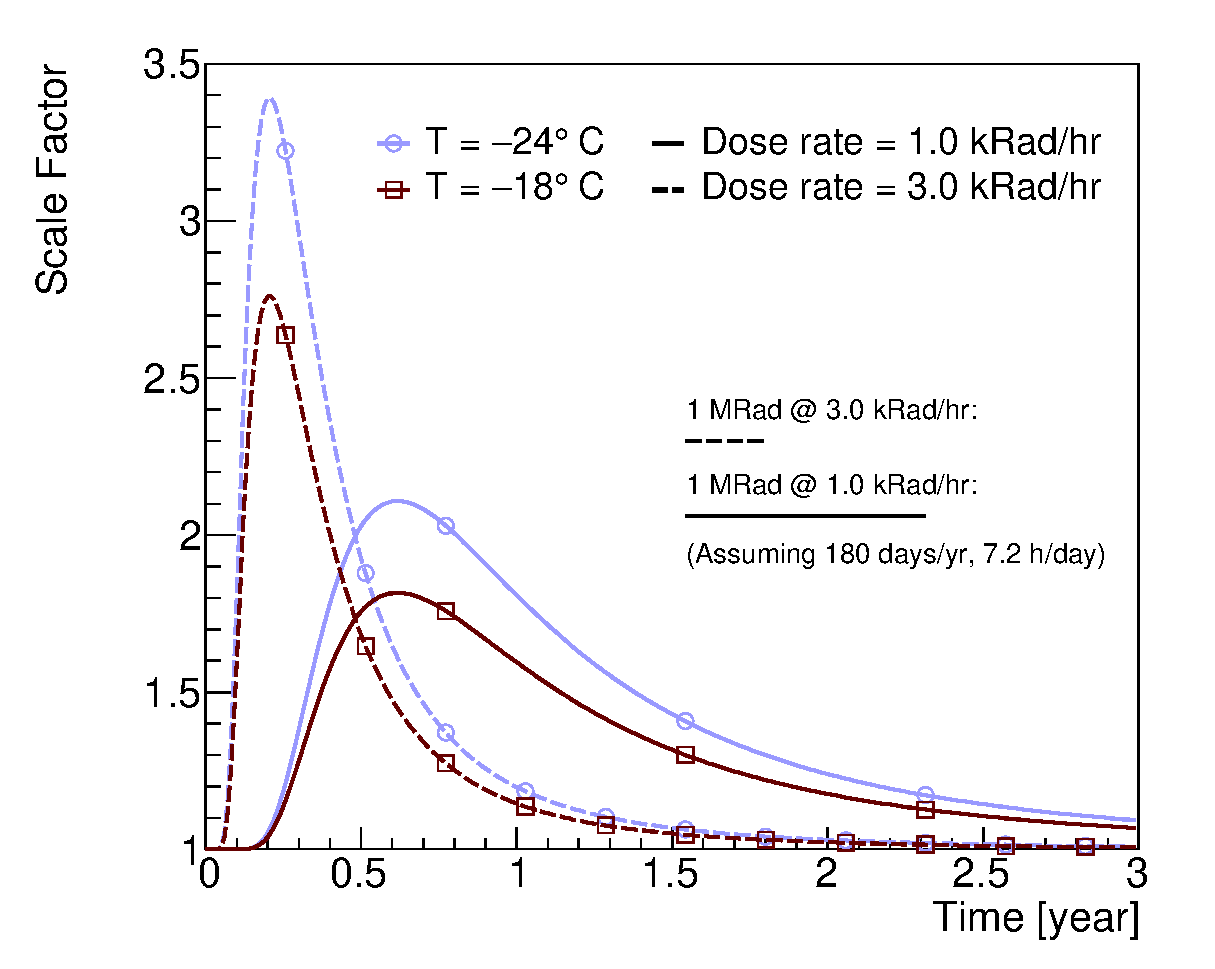
\includegraphics[width=0.6\linewidth]{figures/AbcTidBumpVersionRatesAndTemps_Nominal.eps}
\caption{Parameterization of the impact of the total ionizing dose
on the magnitude of the front-end chip digital current. The current is multiplied by a scale factor
that is modeled as a function of dose rate and temperature, based on experimental data.}
\end{figure}

\subsubsection{Modeling flux and total ionizing dose in endcap modules}

